\documentclass{beamer}
\usetheme{Madrid}

%packages
\usepackage{graphicx}
\usepackage{tikz}
\usepackage{subcaption}
\usepackage{amsmath}
\usepackage[numbers, compress]{natbib}
\bibliographystyle{plainnat}

%graphics
\graphicspath{{./img/}}

%custom commands
\newcommand{\Fcal}{\mathcal{F}}
\newcommand{\Dcal}{\mathcal{D}}

\title{Inferring community characteristics in labelled networks}
\subtitle{IIB Project}
\author{Lawrence Tray}
\institute{Ioannis Kontoyiannis}
\date{\today}

\AtBeginSection[]{
	\begin{frame}
		\vfill
		\centering
		\begin{beamercolorbox}[sep=8pt,center,shadow=true,rounded=true]{title}
			\usebeamerfont{title}\insertsectionhead\par%
		\end{beamercolorbox}
		\vfill
	\end{frame}
}

\begin{document}
	
	\begin{frame}
		\titlepage
	\end{frame}

	\begin{frame}{Overview}
		\tableofcontents
	\end{frame}

	\section{Introduction}
	
	\begin{frame}{Motivation}

	\end{frame}

	\section{Preliminaries}
	
	\begin{frame}{The stochastic block model (SBM)}
		\begin{columns}
			\column{0.5\textwidth}
			Initial parameters:
			\begin{itemize}
				\item $N$ -- number of vertices
				\item $B$ -- number of blocks
			\end{itemize}
			\vspace{1em}
			SBM parameters:
			\begin{itemize}
				\item $b$ -- block membership vector
				\item $e$ -- block connectivity matrix
				\item $k$ -- degree sequence
			\end{itemize}
			
			\begin{equation}
				A \sim \textrm{DC-SBM}_{\textrm{MC}}(b, e, k)
			\end{equation}
			
			\column{0.5\textwidth}
			
			\begin{figure}
				\includegraphics[width=0.8\linewidth]{polbooks-graph}
				\caption{Typical SBM}
			\end{figure}
		\end{columns}
	\end{frame}

	\section{The feature-first block model}
	\begin{frame}{The feature-first block model (FFBM)}
		\begin{figure}[!h]
			\centering
			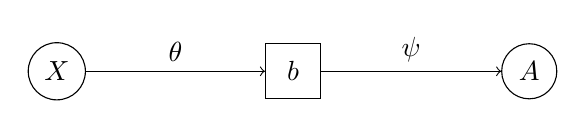
\begin{tikzpicture}[
				roundnode/.style={circle, draw=black, minimum size=7mm},
				squarednode/.style={rectangle, draw=black, minimum size=7mm}
				]
				% nodes
				\node[roundnode] (X) at (0, 0) {$X$};
				\node[squarednode] (b) at (3, 0) {$b$};
				\node[roundnode] (A) at (6, 0) {$A$};
				
				% arrows
				\draw[->] (X.east) -- node[above] {$\theta$} (b.west);
				\draw[->] (b.east) -- node[above] {$\psi$}(A.west);
			\end{tikzpicture}
			\caption{The feature-first block model (FFBM)}
			\label{fig:ffbm}
		\end{figure}
	
		\begin{align}
			p(b|X; \theta) &= \prod_{i \in [N]} \phi_{b_i} (x_i; \theta)
			= \prod_{i \in [N]} \frac{\exp (w_{b_i}^T x_i)}{\sum_{k \in [B]} \exp (w_k^T x_i) } \\ \nonumber \\
			p(A|b; \psi) &\sim \textrm{DC-SBM}_{\textrm{MC}} (b, \psi_e, \psi_k)
		\end{align}
	\end{frame}

	\section{Inference}
	\begin{frame}{Inference procedure}
		We want to draw:
		\begin{equation}
			\theta^{(t)} \sim p(\theta| A, X).
		\end{equation}
		We achieve this by:
		\begin{align}
			b^{(t)} &\sim p \Big( b| A, X \Big) \\
			\theta^{(t)} &\sim p \Big( \theta| X, b^{(t)} \Big)
		\end{align}
	\end{frame}

	\begin{frame}{Metropolis-Hastings (reference) \cite{hastings-alg}}
		We want to draw samples for $\left\{ x^{(t)} \right\}$ from some distribution,
		\begin{equation}
			\pi^*(x) \propto \pi(x).
		\end{equation}
		Just need to be able to evaluate $\pi(x)$ point-wise and simulate from a proposal $q(x, x')$. If we accept each proposal with probability,
		\begin{equation}
			\alpha(x, x') = \min \left( \frac{\pi(x') q(x', x)}{\pi(x) q(x, x')} , 1 \right),
			\label{eqn:mh-accept}
		\end{equation}
		then the resulting Markov chain is in detailed balance with $\pi(x)$.
	\end{frame}
	
	\begin{frame}{Sampling sequence}
		\begin{figure}[!h]
			\centering
			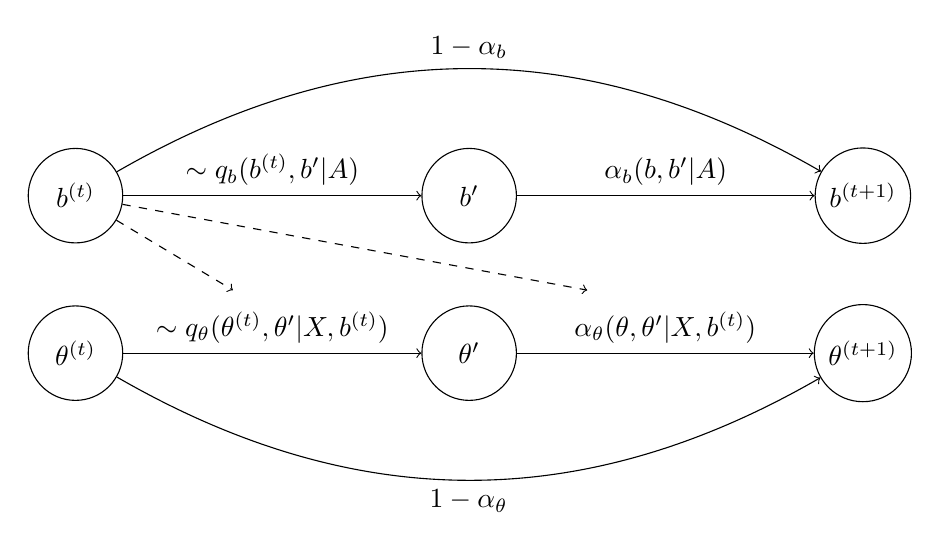
\begin{tikzpicture}[
				scale=1.0, every node/.style={transform shape},
				roundnode/.style={circle, draw=black, minimum size=12mm},
				squarednode/.style={rectangle, draw=black, minimum size=12mm}
				]
				% nodes
				\node[roundnode] (b0) at (0, 2) {$b^{(t)}$};
				\node[roundnode] (b1) at (5, 2) {$b'$};
				\node[roundnode] (b2) at (10, 2) {$b^{(t+1)}$};
				\node[roundnode] (t0) at (0, 0) {$\theta^{(t)}$};
				\node[roundnode] (t1) at (5, 0) {$\theta'$};
				\node[roundnode] (t2) at (10, 0) {$\theta^{(t+1)}$};
				
				% arrows
				\draw[->] (b0) to node[above] {$\sim q_b(b^{(t)}, b' | A)$} (b1);
				\draw[->] (b1) to node[above] {$\alpha_b (b, b' | A)$} (b2);
				\draw[->] (b0) [out=30, in=150] to node[above] {$1-\alpha_b$} (b2);
				
				\draw[->] (t0) to node[above] {$\sim q_\theta(\theta^{(t)}, \theta' | X, b^{(t)})$} (t1);
				\draw[->] (t1) to node[above] {$\alpha_\theta (\theta, \theta' | X, b^{(t)})$} (t2);
				\draw[->] (t0) [out=-30, in=-150] to node[below] {$1-\alpha_\theta$} (t2);
				
				\draw[dashed, ->] (b0) to (2, 0.8);
				\draw[dashed, ->] (b0) to (6.5, 0.8);
				
			\end{tikzpicture}
			\caption{Sampling sequence.}
			\label{fig:samp-sequence}
		\end{figure}
	\end{frame}

	\begin{frame}{Speed up computation}
		content...
	\end{frame}

	\begin{frame}{Dimensionality Reduction}
	\end{frame}

	\section{Experiments}
	
	\begin{frame}{Political Books}
		\begin{figure}
			\includegraphics[width=0.4\linewidth]{polbooks-graph.png}
			\caption{Polbooks}
		\end{figure}
	\end{frame}

	\begin{frame}{References}
		\bibliography{presentation.bib}
	\end{frame}

\end{document}
